\chapter{INTRODUCTION}
\onehalfspacing
\setlength{\parindent}{0pt}

\section{History}
Gravitational waves are predicted by Einstein’s general theory of relativity published in 1916 \cite{einstein1916naherungsweise} and are the ripples in space-time fabric generated by massive objects. However, their direct detection was a scientific problem which took approximately a century. There has been no direct observation of gravitational waves until September 14, 2015, when LIGO announced its detection of gravitational waves \citep{abbott2016observation} resulting from the binary black hole merger. The later discoveries such as the binary neutron stars have helped confirm the existence of gravitational waves and ushered in a new age in the understanding of the cosmos in a new paradigm.
\section{Gravitational Waves}
% Gravitational waves\footnote{\url{https://www.ligo.org/science/overview.php}} are 'ripples' in space-time caused by some of the most violent and energetic processes in the Universe. Einstein's mathematics showed that massive accelerating objects (things like neutron stars or black holes orbiting each other) would disrupt space-time in such a way that 'waves' of undulating space-time would propagate in all directions away from the source. These cosmic ripples would travel at the speed of light, carrying with them information about their origins, as well as clues to the nature of gravity itself.
Gravitational waves are ripples in space-time which are produced by some of the most violent events in the Universe. In Einstein’s mathematics \cite{einstein1916naherungsweise} when large accelerating objects such as neutron stars or black holes are revolving around one another they would distort space-time in a way that created waves of fluctuating space-time that would radiate out from the source in all directions \citep{thesis}\citep{Hughes_2009}. These waves would move with the speed of light and along with the information about their source.
\section{Black Hole}
A black hole is an astronomical object in which the gravitational force is so intense that no matter or radiation can escape from the region known as the event horizon. According to general relativity, if a mass is sufficiently compact it can warp space to create a black hole. Black holes are believed to be created at the death of a massive star through the process of stellar collapse. When a star has used up the nuclear fuel in its core, it can no longer maintain the outward pressure necessary to counteract gravity and the star collapses under its own weight. If the mass of the stellar core reaches the critical value, it will shrink to a point of density, turning into a black hole.

\section{Binary Black Hole}
Binary black holes are pairs of black holes that orbit around a common center of mass due to their gravitational attraction. As they orbit each other, they emit gravitational waves, which cause them to spiral closer and closer together (Fig \ref{fig:phase}). Eventually, the two black holes will merge, releasing a tremendous amount of energy in the form of gravitational waves. The existence of stellar-mass binary black holes was finally confirmed when LIGO detected GW150914, a distinctive gravitational wave signature of two merging stellar-mass black holes of around 30 $M_\odot$ each, occurring about 1.3 billion light-years away \citep{abbott2016observation}.

\section{Neutron Star}
Neutron stars are formed when a massive star runs out of fuel and collapses. The very central region of the star core collapses, crushing together every proton and electron into a neutron. If the core of the collapsing star is between about 1 and 3 $M_\odot$, these newly-created neutrons can stop the collapse, leaving behind a neutron star (Stars with higher masses will continue to collapse into stellar-mass black holes). Neutron stars are the smallest and densest known class of stellar objects. Most neutron stars are observed as pulsars. Pulsars are rotating neutron stars observed to have pulses of radiation at very regular intervals that typically range from milliseconds to seconds. Pulsars have very strong magnetic fields which funnel jets of particles out along the two magnetic poles. These accelerated particles produce very powerful beams of light.

\section{Binary Neutron Star}
Binary neutron stars are pairs of neutron stars that orbit around a common center of mass due to their gravitational attraction. Binary neutron stars are some of the most energetic objects in the universe. As they orbit each other, they emit gravitational waves, which cause them to spiral closer and closer together. Eventually, the two neutron stars will merge, releasing a tremendous amount of energy in the form of gravitational waves and electromagnetic radiation. The first binary pulsar, PSR B1913+16, was discovered in 1974 by Hulse and Taylor \citep{1975ApJ...195L..51H}, who won the Nobel Prize in Physics in 1993 for their work on this system. On August 17, 2017, the LIGO and VIRGO detectors observed the GW170817  gravitational wave signal \citep{2017ApJ...848L..12A}, emanating from the elliptical galaxy NGC 4993, resulting from the final moments of a binary neutron star pair's inspiral and subsequent merger.

\section{Sources of Gravitational Waves}
The Gravitational Waves are produced by the acceleration of massive bodies and spread out in space at the speed of light, conveying information about their source and the characteristics of gravity. 
Gravitational wave sources fall into four main categories:
\vspace{0.2cm}

\subsection{Short-lived and well-modeled Sources}
This category consists mostly of compact object pairs on tight orbits, such as neutron stars or black holes. These systems emit gravitational waves in three distinct phases: inspiral, merger, and ringdown. Because of their predictability, they are among the prime targets for gravitational wave observatories like as LIGO, VIRGO, and KAGRA.
\vspace{0.2cm}

\subsection{Short-lived and Poorly Understood Sources}
This category includes events such as supernovae and long-duration gamma-ray bursts. These astrophysical events will likely create gravitational waves due to asymmetries in their explosive processes. Supernovae occur when a big star's nuclear fuel becomes exhausted, causing its core to collapse under gravity and explode. Asymmetric core collapse can produce gravitational waves. Gamma-ray bursts are long-duration GRBs related to enormous star deaths, which might lead to supernovae or the merging of compact objects \citep{nasaGammaRayBursts2023}\citep{Troja2022-bo}. Gravitational waves from GRBs may originate from the very intense and asymmetric mechanisms that fuel these explosions.
\vspace{0.2cm}

\subsection{Long-lived and Well-modeled Sources}
Long-lived sources of gravitational waves are usually periodic and stable over time, making them easier to analyze and detect. Rapidly spinning neutron stars do not have an axisymmetric mass distribution around their rotation axis. As they spin, these stars generate nearly monochromatic gravitational waves with a frequency proportional to their rotation period. In some fast-rotating neutron stars, certain oscillation modes known as r-modes can become unstable and grow over time \citep{Ho2018-ip}.
\vspace{0.2cm}

\subsection{Long-lived, Diffuse Sources}
This category refers to gravitational wave backgrounds that are diffuse and long-lived, resulting from a combination of several unresolved sources or cosmic events in the early universe. Primordial gravitational waves are thought to have originated during the early universe's inflationary phase, a period of fast expansion that might have caused ripples in spacetime \citep{Guzzetti2016-qv}. Detecting these extremely low-frequency gravitational waves might reveal information on the mechanics of the early cosmos, especially the mechanism of inflation. If hypothetical cosmic strings, which are topological imperfections in the fabric of spacetime, form loops, and snap, they may create gravitational waves. These occurrences may contribute to a stochastic backdrop of gravitational waves \citep{PhysRevD.97.102002}.

% \begin{figure}[h]
%     \centering
%     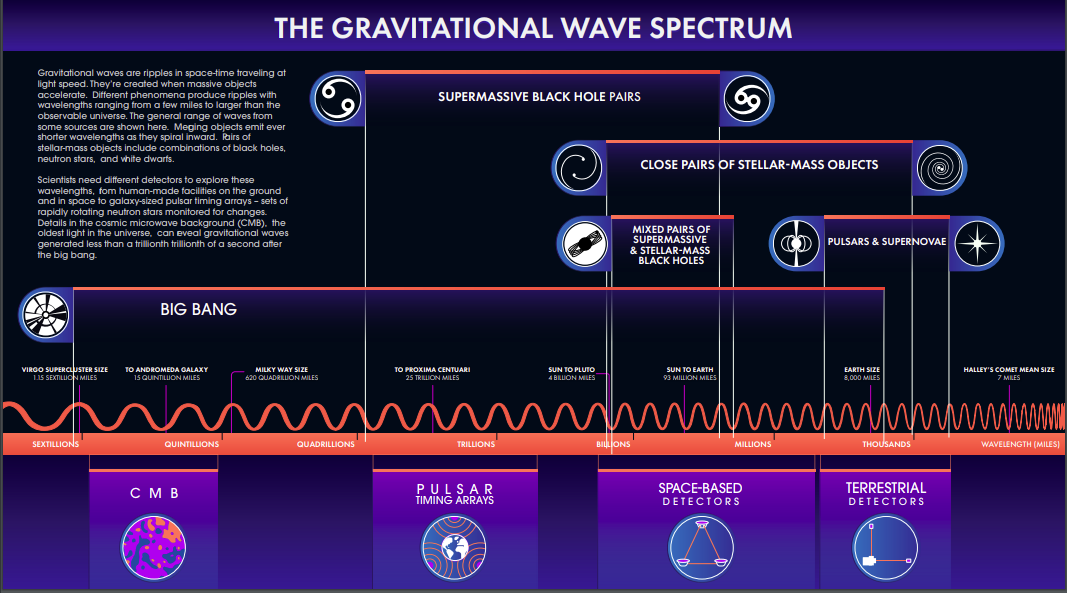
\includegraphics[width=4in]{images_/spectrum.png}
%     \caption{Gravitational-wave spectrum (credit: NASA)}
%     \label{fig:spectrum}
% \end{figure}

\section{Types of Gravitational Waves}
The classification of gravitational waves is based on the nature of their sources, the duration of their signals, and their waveform characteristics. There are several types of gravitational waves, each associated with different astrophysical sources and characteristics.
Gravitational waves are categorized into four main groups based on their sources:
% \vspace{0.2cm}

\subsection{Continuous Gravitational Waves} 
Continuous gravitational waves are emitted by fast-rotating, non-axisymmetric objects such as neutron stars. These objects may have small deformations on their surfaces, or they may be subject to internal instabilities that lead them to emit gravitational waves continuously over a long period. The source of continuous gravitational waves is usually a neutron star that is not exactly spherical. As it spins, any asymmetry in its mass distribution causes a periodic disturbance in spacetime, resulting in gravitational waves with a frequency proportional to its rotation rate. The gravitational waves produced are almost monochromatic, which means their frequency is generally consistent across time. This frequency may be somewhat altered by the star's interactions with its surroundings or change in its rotation.
\vspace{0.2cm}

\subsection{Compact Binary Inspiral Gravitational Waves} 

Compact binary inspiral gravitational waves thus results from inspiral and merger of two compact objects, neutron stars or black holes. These are some of the best-understood sources of gravitational waves. The sources are normally binary systems of neutron stars, black hole or both neutron star and black hole. These objects move in their orbits and in the process, they emit gravitational waves whereby they lose energy and hence their orbit shrinks and their orbital frequency increases. The produced gravitational waves have chirp signal in which both frequency and amplitude rise as the objects come closer. The waveform consists of three phases: Spiral, merger and ringdown. The inspiral is long, well modeled, and less energetic in contrast with the merger which is short, less modelled, and more energetic and the final ringdown, whereby the object created by the merger becomes stable.
\vspace{0.2cm}

\subsection{Stochastic Gravitational Waves} 
Stochastic gravitational waves are low-frequency gravitational waves from unresolved, disparate sources that overlap with each other: This background is similar to the cosmic microwave background radiation but for the gravitational waves. The stochastic background can have various astrophysical origins, such as a large number of low luminosity, unresolved mergers, core-collapse supernovae or the early universe; inflation, or cosmic strings. These sources contribute to a stochastic/ stochastic background of gravitational waves. Unlike the precise signals from individual events, the stochastic background is a random noise-like signal. Its detection is done with statistical measures other than the actual recognition of certain waveforms.
\vspace{0.2cm}

\subsection{Burst Gravitational Waves}
The burst gravitational waves are short-lived and transient signals that are due to sudden and catastrophic phenomena in the universe. Such events are often stochastic and might pose a problem in terms of modeling. Burst gravitational waves are normally associated with a core-collapse supernova, neutron star mergers, gamma-ray bursts, or another astrophysical catastrophe. These sources create ripples in the space-time fabric over a very short duration and therefore create a burst signal. The signal can have different duration, frequency, and amplitude depending on the source of the signal.

\section{Phase of Gravitational Waves}
The phase of a gravitational wave signal is the time evolution of the wave's oscillation. Gravitational wave signals can be divided into three phases (Fig \ref{fig:phase}):
   \begin{figure}[h]
        \centering
        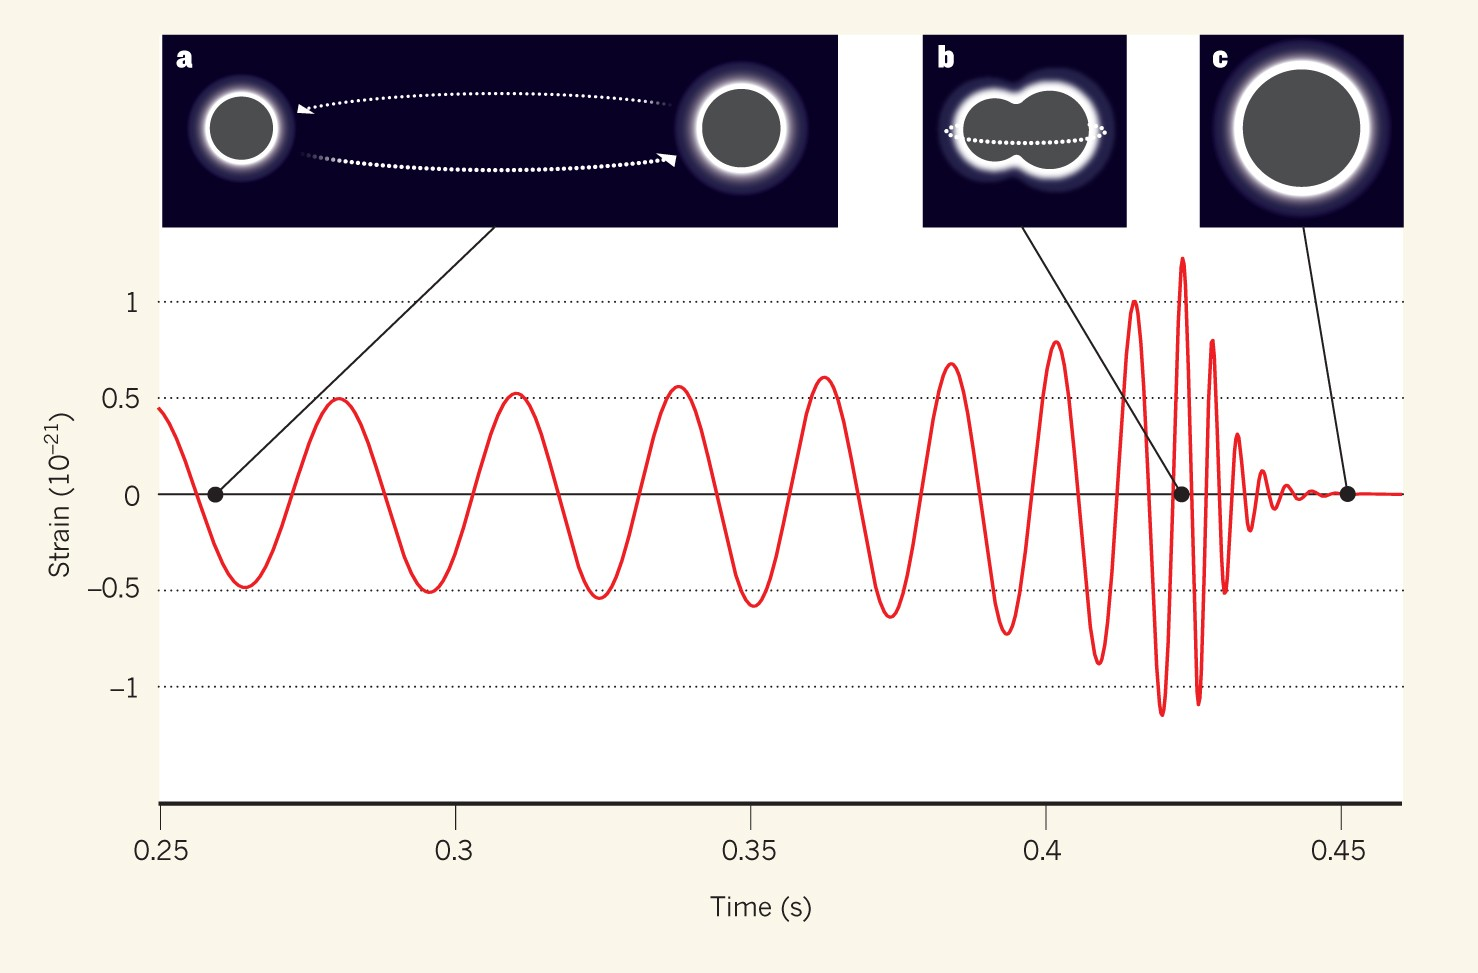
\includegraphics[width=4.5in]{images_/phase.jpg}
        \caption{A gravitational wave from merging black holes.(a) Inspiral Phase.(b) Merger Phase.(c) Ringdown Phase. Source: \citep{Miller2016}}
        \label{fig:phase}
    \end{figure}

    \subsection{Inspiral}
    The inspiral phase is the first phase of the gravitational wave signal in which two compact objects, such as neutron stars or black holes, gradually approach each other and orbit around their common center of mass because of the emission of gravitational radiation. In the inspiral phase, the GWS increases in both frequency as well as amplitude as the objects come closer to each other. This phase can continue for quite a long duration, especially in systems of lower mass, and is reasonably well explained by the post-Newtonian approximations of general relativity. When the objects are in orbit around each other the energy is radiated away in the form of gravitational waves and the separation of the objects reduces causing the orbits to become faster and the gravitational waves to become stronger. The rising of the frequency and the amplitude of the signal in a chirp-like manner is characteristic of this phase.
    
    \subsection{Merger}
    The merger phase is the most complex and the most violent phase of the gravitational wave signal and it is the phase where the two objects merge and form one object. The last phase of a binary’s life cycle is the merger phase as the frequency and amplitude rise steeply and steeply to the maximum values of the wave signal. This phase is very short and it can last for just a few milliseconds but the gravitational fields here are very strong and this is where general relativity’s nonlinear effects start to manifest themselves. It is within this process that the two objects’ gravitational fields are most intense and engage in a dance that is best explained through the numerical relativity simulations. The nature of the signal – frequency and its time variation – is defined by properties of the merging objects themselves, such as their masses, spins, and, in case the objects are neutron stars, the equation of state for these stars.
    
    \subsection{Ringdown} 
    The ringdown phase occurs after the merger and in essence, it is the period during which a newly-formed object settles down and becomes a black hole. This phase is characterised by exponential damping oscillations which are referred to as the quasinormal modes. The ringdown signal is a series of exponentially damped oscillations at a certain frequency which is determined by the mass and spin of the last formed black hole. These oscillations reduce in amplitude over time release of the rest of the distortions by the black hole.
    % \begin{figure}[h]
    %     \centering
    %     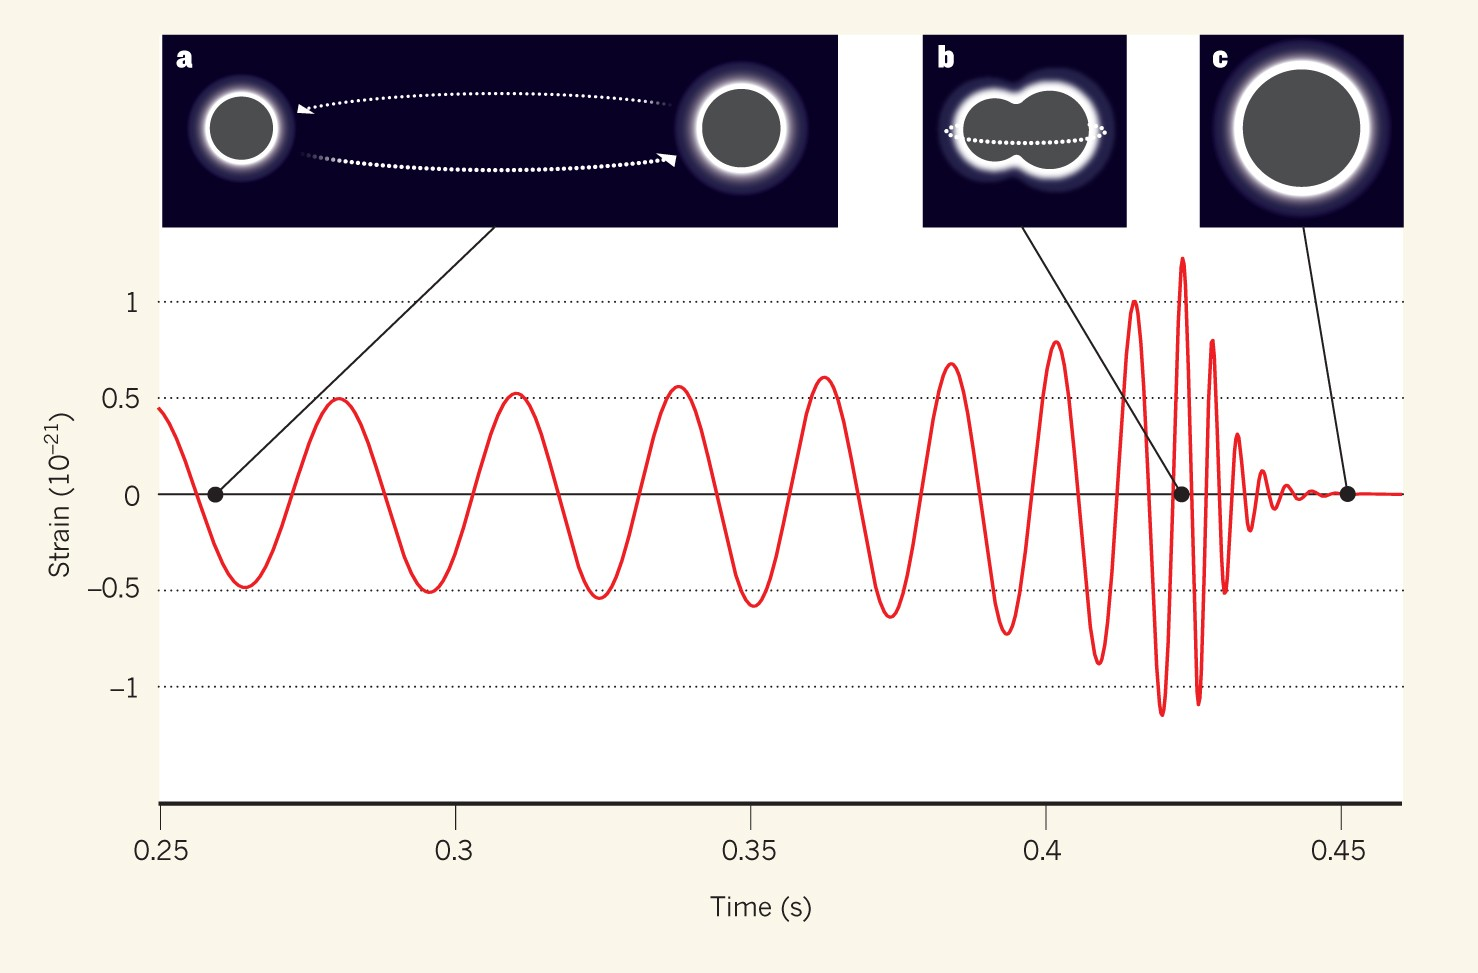
\includegraphics[width=4.5in]{images_/phase.jpg}
    %     \caption{A gravitational wave from merging black holes.(a) Inspiral Phase.(b) Merger Phase.(c) Ringdown Phase. Source: \citep{Miller2016}}
    %     \label{fig:phase}
    % \end{figure}
\section{Method of Gravitational Wave Detection}
Gravitational waves can be detected using two main methods: laser interferometry and pulsar timing arrays.
    
\begin{enumerate}
    \item \textbf{Laser Interferometry:} This method involves measuring tiny changes in the distance between two mirrors separated by a long distance (Fig: \ref{fig:interferometer}). When a gravitational wave passes through the detector, it stretches and squeezes space, causing slight changes in the mirror distance. Lasers and highly sensitive detectors are used to measure these changes with great precision. Laser interferometry detectors include LIGO, VIRGO, GEO600 and KAGRA.
    \begin{figure}
        \centering
        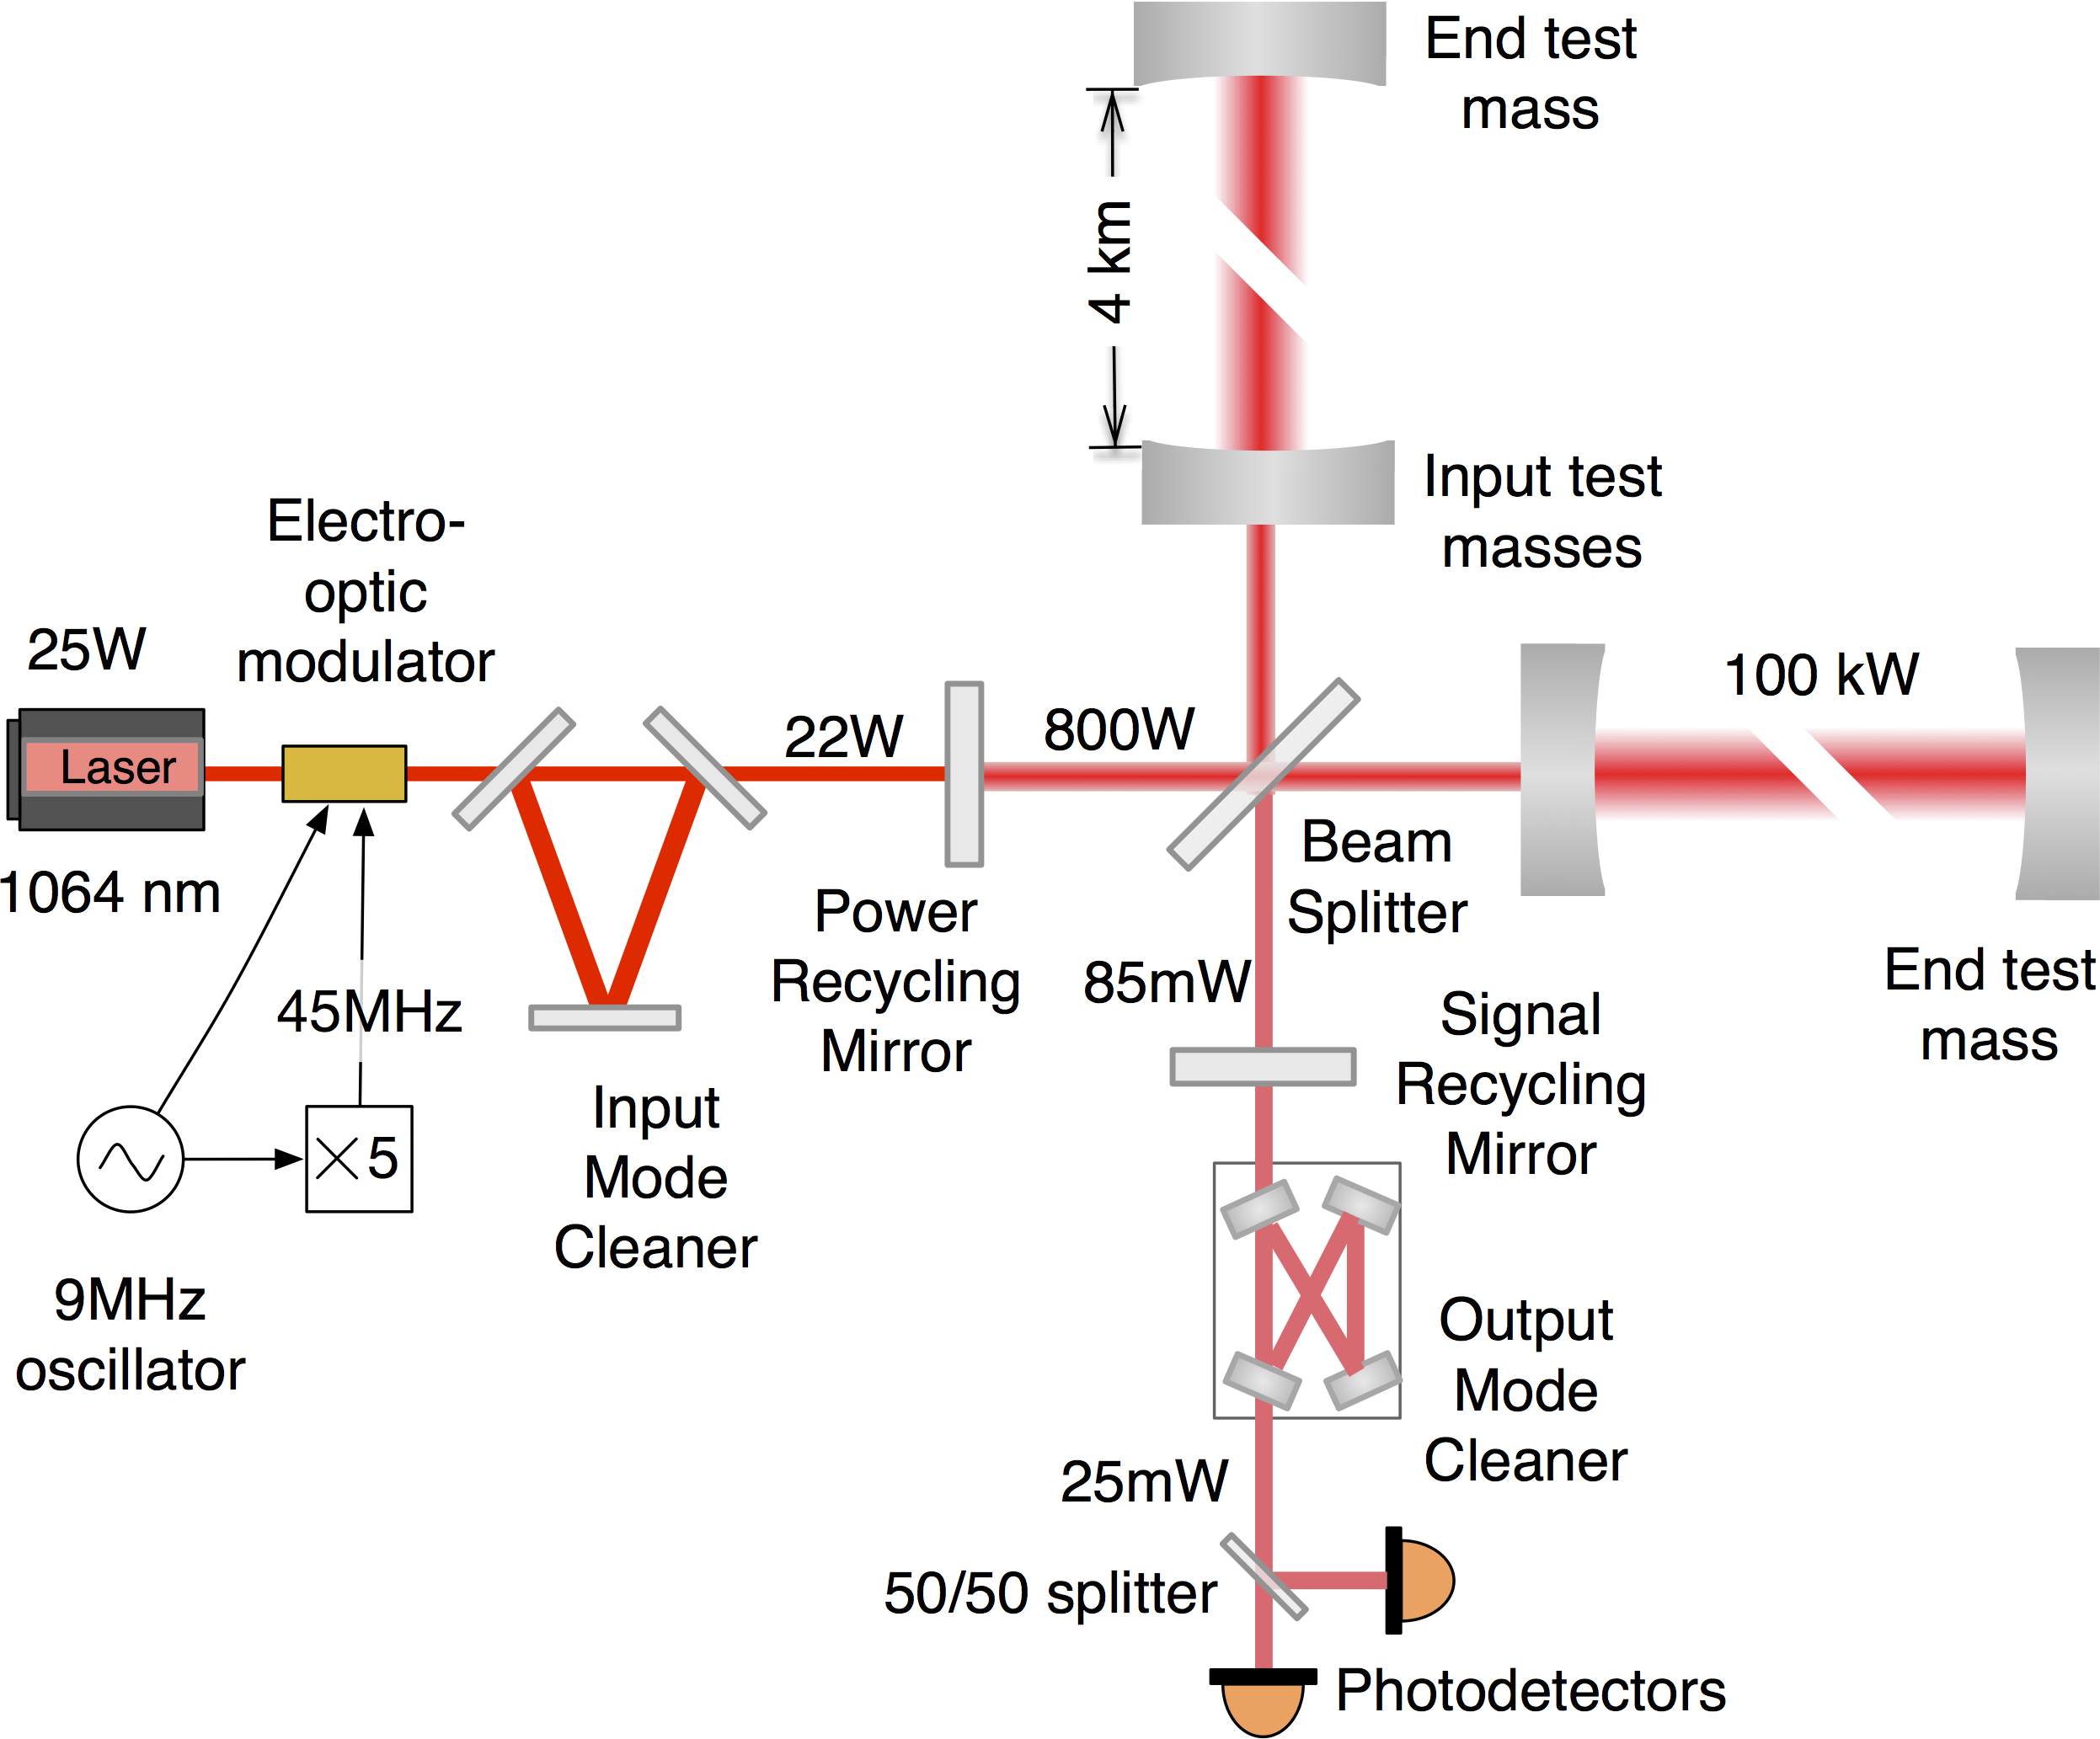
\includegraphics[width=0.65\linewidth]{images_/interferometer.png}
        \caption{LIGO's Interferometer. Source: \citep{PhysRevD.93.112004}}
        \label{fig:interferometer}
    \end{figure}
    
    \item \textbf{Pulsar Timing Arrays:} Pulsar timing arrays are networks of radio telescopes that are used to monitor the arrival times of pulses from millisecond pulsars. PTAs are less sensitive than laser interferometer gravitational wave detectors. However, PTAs can detect lower-frequency gravitational waves, which makes them well-suited for detecting gravitational waves from sources such as supermassive black hole mergers and cosmic strings. Examples are NANOGrav, EPTA and IPTA.
    
\end{enumerate}
% \section{Noises}
% "Noise" is unwanted and random fluctuations or signals that can obscure or mask the true gravitational wave signals. Some common sources of noise in gravitational wave detectors include:
%     \subsection{Seismic Noise} 
%     Ground vibrations caused by seismic activity, as well as other environmental factors like wind and temperature fluctuations, can introduce noise into the detector. To filter out these disturbances, the optical components are suspended to a series of several pendulums, each hanging from the above. 
%    \subsection{Thermal Noise} 
%    This source of noise in gravitational wave detectors is associated with the thermal vibrations of the mirrors and their suspensions. The steel wire that suspends the mirror is typically at room temperature, in thermal equilibrium with the surrounding environment. These thermal fluctuations can induce motion in the mirror, which, in turn, changes the length of the interferometer's arm.
%     \subsection{Quantum Noise}
%     Quantum mechanics imposes fundamental limits on the precision of measurements. Quantum noise arises due to the inherent uncertainty in position and momentum of particles. It can affect the accuracy of interferometric measurements used in many gravitational wave detectors.
%     \subsection{Shot Noise} 
%     Photon shot noise is the major limiting source of disturbance at frequencies above 200 Hz and results from the finite number of photons arriving at the photo-detector. Shot noise can be reduced by increasing the laser power. In order to be able to detect gravitational waves with frequency 100 Hz, the intensity of the laser would need to be of the order of 100 W, a value beyond the capability of any existing continuous laser.
%     \subsection{Mirror Coating Noise} 
%     The reflective coatings on mirrors used in interferometers can introduce noise when they fluctuate or deform, affecting the quality of the laser beam's reflection.
%     \subsection{Electromagnetic Interference (EMI)} 
%     External electromagnetic signals, including radio frequency interference (RFI) and electronic noise, can interfere with detector operations.
\section{Noises}

Noise refers to unwanted and random fluctuations or signals that can obscure or mask the true gravitational wave signals in detectors. The sensitivity and accuracy of gravitational wave detectors are significantly influenced by various types of noise. Understanding and mitigating these noise sources are crucial for accurate detections. Common sources of noise (Fig: \ref{fig:noises}) include:

\subsection{Seismic Noise} Seismic noise arises from ground vibrations caused by seismic activity, as well as environmental factors like wind, ocean waves, and human activities such as traffic and construction. These vibrations can be transmitted to the interferometer's components, particularly the mirrors, causing distortions that mimic or obscure gravitational wave signals. To reduce the impact of seismic noise, the optical components in detectors are suspended by multiple pendulums in a series, each hanging from the one above it. This sophisticated suspension system acts as a mechanical filter, isolating the mirrors from ground vibrations, especially at higher frequencies.

\subsection{Thermal Noise} Thermal noise is associated with the random thermal vibrations of the mirrors and their suspensions, which are typically made of materials like fused silica or steel. Even at room temperature, these materials experience microscopic vibrations due to thermal energy, leading to small, random movements of the mirrors. These movements can change the length of the interferometer's arms, introducing noise into the measurements. To mitigate thermal noise, gravitational wave detectors often operate at cryogenic temperatures, where thermal vibrations are significantly reduced. Additionally, advanced materials and coatings are used to minimize the mechanical losses that contribute to thermal noise.

\subsection{Quantum Noise} Quantum noise is a fundamental limitation imposed by quantum mechanics on the precision of measurements. It arises due to the Heisenberg uncertainty principle, which limits the simultaneous accuracy of position and momentum measurements. In the context of gravitational wave detectors, quantum noise primarily manifests as two effects: photon shot noise and radiation pressure noise. Photon shot noise, caused by the discrete nature of light, becomes significant at high frequencies, while radiation pressure noise, due to the fluctuating force exerted by photons on the mirrors, dominates at low frequencies. Techniques like quantum squeezing, where the quantum uncertainties are redistributed between variables, are employed to reduce quantum noise and enhance detector sensitivity.
\begin{figure}[h]
        \centering
        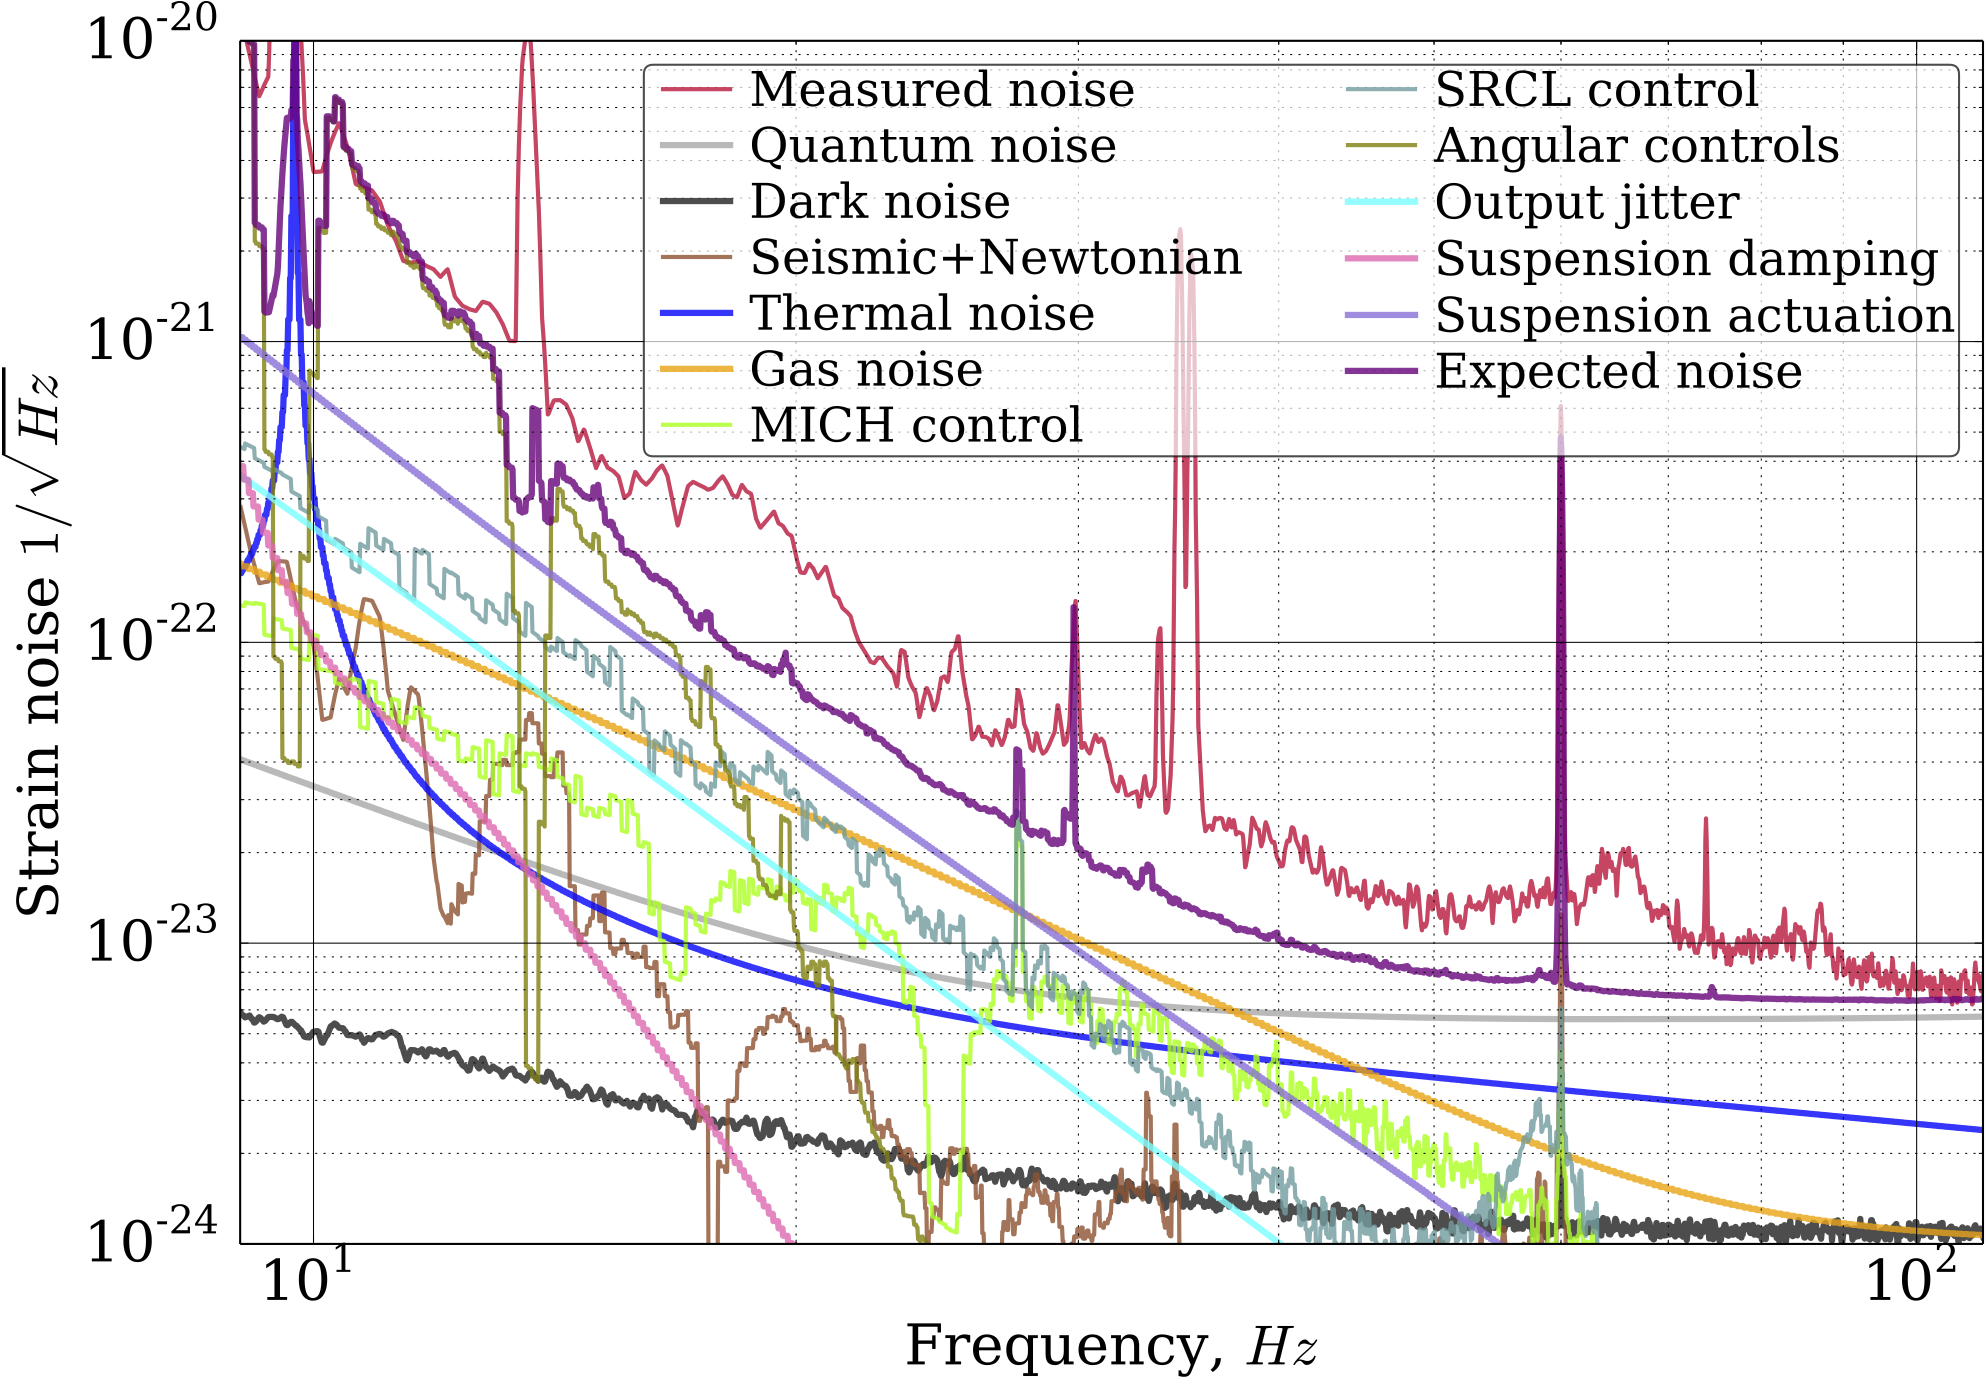
\includegraphics[width=4.5in]{images_/noise.png}
        \caption{ Accounting of sources of noise that combine to form the limiting sensitivity of the detectors. Source: \citep{PhysRevD.93.112004}}
        \label{fig:noises}
\end{figure}

\subsection{Mirror Coating Noise} Mirror coating noise is introduced by the reflective coatings on the mirrors used in interferometers. These coatings, typically made of materials like silica or tantala, are essential for reflecting the laser beam in the interferometer. However, thermal fluctuations and mechanical stress in the coating layers can cause them to deform or fluctuate, leading to noise in the reflected laser signal. This noise is particularly challenging to mitigate, as it is closely tied to the optical properties and thickness of the coatings. Research into advanced coating materials and techniques, such as crystalline coatings, is ongoing to reduce this type of noise.

\subsection{Electromagnetic Interference (EMI)} Electromagnetic interference is caused by external electromagnetic signals, such as radio frequency interference from communication devices, power lines, or electronic noise from nearby equipment. EMI can couple into the sensitive electronics of the detector, leading to spurious signals that mimic or obscure gravitational wave events. To protect against EMI, gravitational wave detectors are often housed in shielded environments with careful attention to grounding and cabling. Additionally, filters and isolation techniques are employed to prevent external electromagnetic signals from interfering with the detector's operations.
    % \begin{figure}[h]
    %     \centering
    %     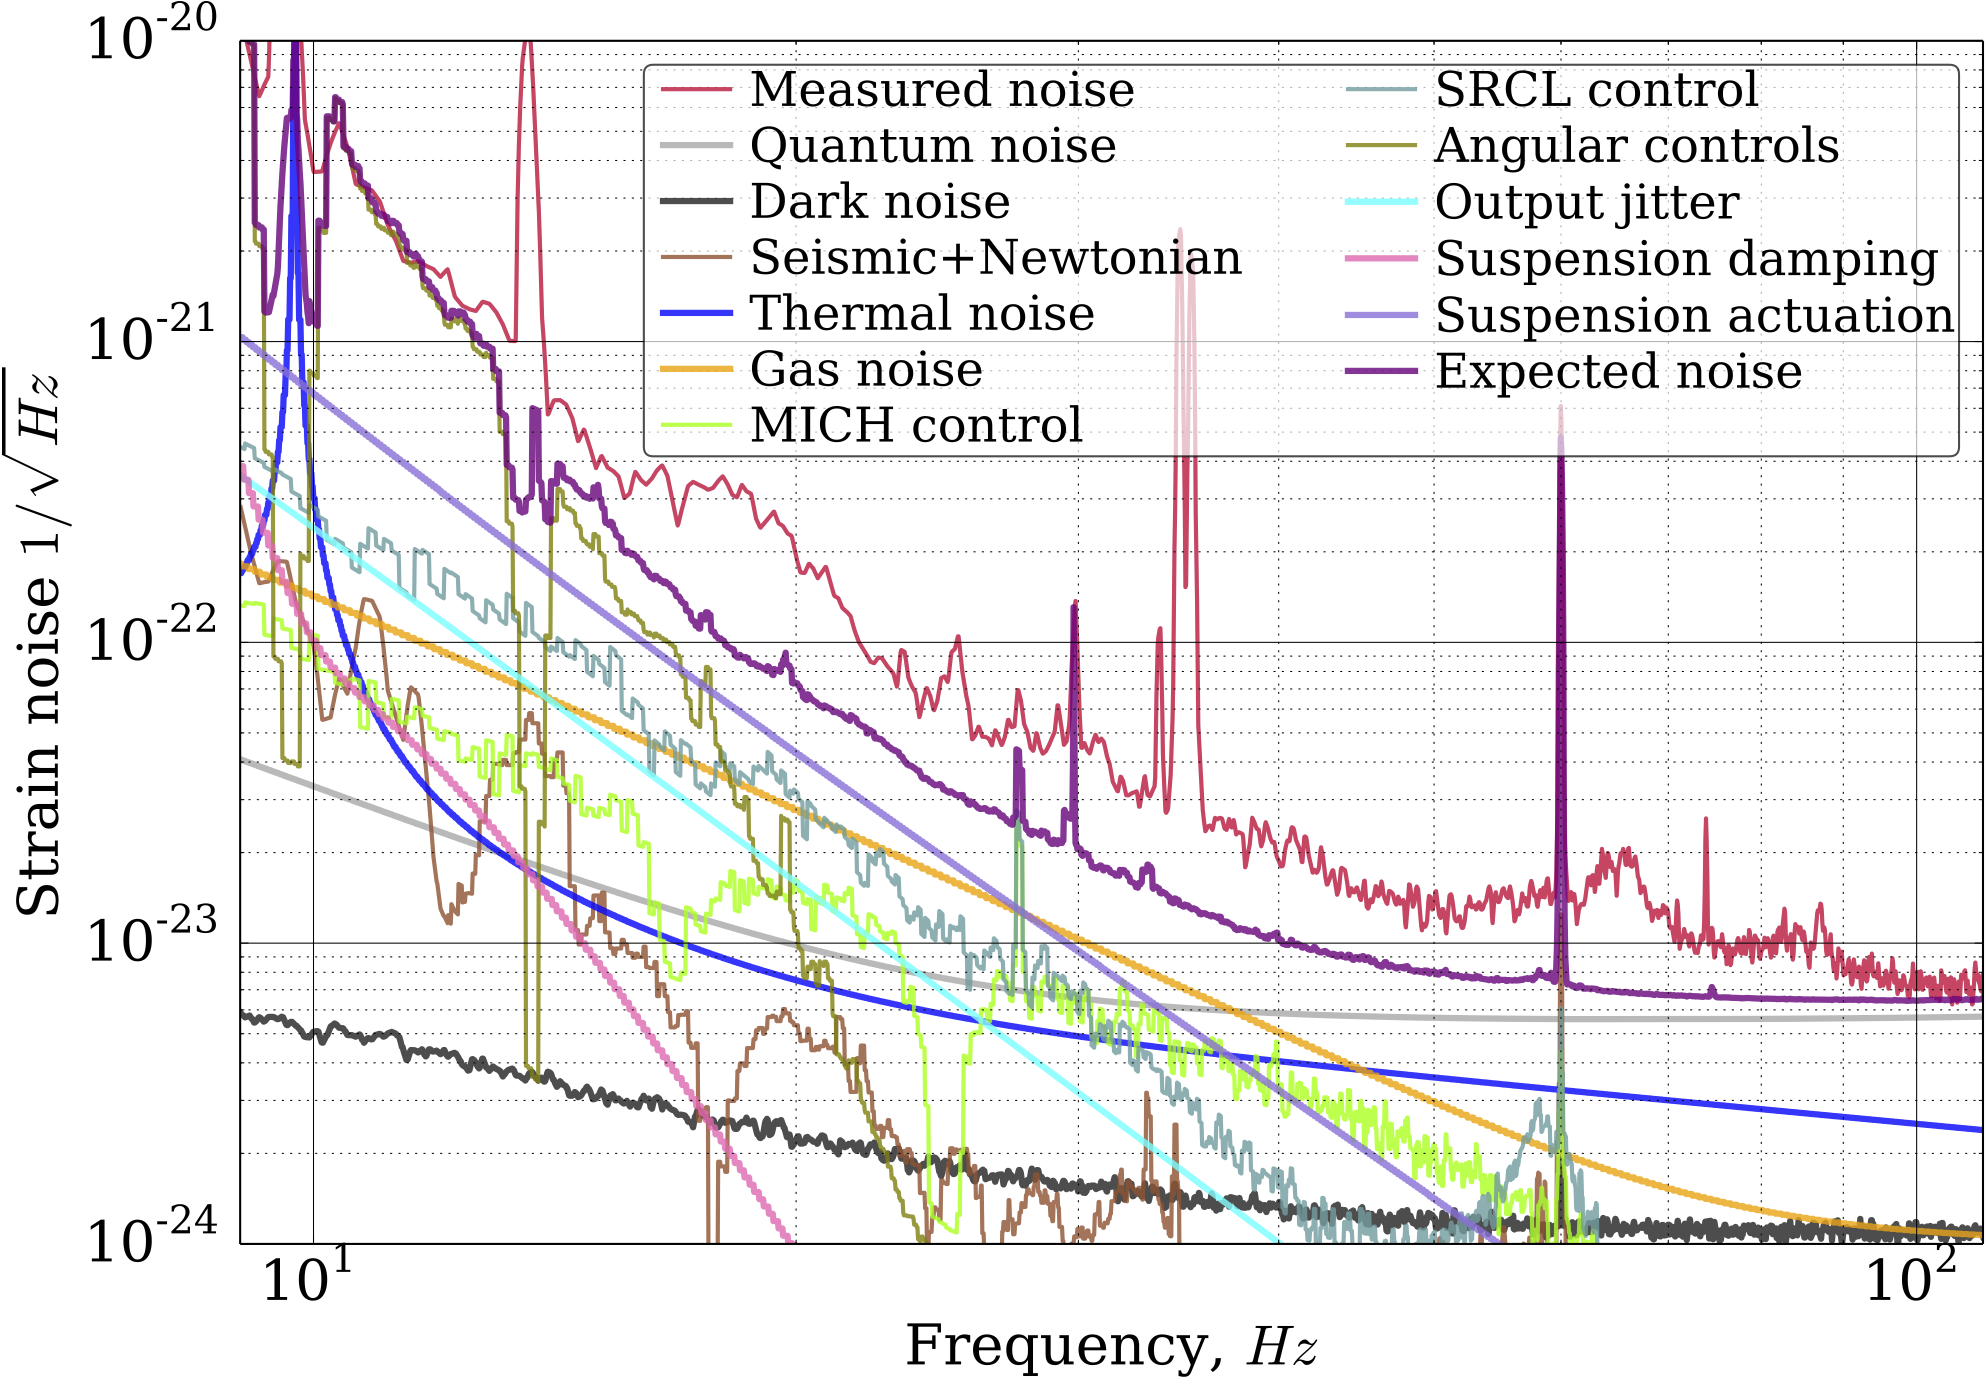
\includegraphics[width=4.5in]{images_/noise.png}
    %     \caption{ Accounting of sources of noise that combine to form the limiting sensitivity of the detectors. Source: \citep{PhysRevD.93.112004}}
    %     \label{fig:noises}
    % \end{figure}

\section{GW170817}
The Gravitational Wave Signal GW170817 was detected on August 17, 2017 by the Advanced LIGO and VIRGO Observatories \citep{2017ApJ...848L..12A}. GW170817 signal is produced from the collision of binary neutron stars. This GW signal is so unique that only 1.7 second after the detection of the signal, Fermi Gamma-ray Burst Monitor (GBM) and the Anticoincidence Shield for the Spectrometer for the International Gamma-Ray Astrophysics Laboratory (INTEGRAL SPI-ACS) detected a short $\gamma$-ray burst GRB 170817A \citep{Savchenko_2017}. For many decades, it had been suspected that these short $\gamma$-ray burst were produced by the merger of two neutron stars or a neutron star and a black hole. However, the detection of the GW signal with EM rays burst provides the first direct evidence of a link between these mergers and short $\gamma$-ray bursts called Kilonovae \citep{2017ApJ...848L..12A}. This unprecedented joint gravitational and electromagnetic observation provides insight into astrophysics, dense matter, gravitation, and cosmology.
\section{GW190521}
The Gravitational Wave Signal GW190521 was detected on May 21, 2019 by the LIGO and VIRGO detectors. It was produced from the merger of two intermediate mass black holes of each mass 85 and 66 $M_\odot$ with mass equivalent to 142 $M_\odot$. The remaining 9 $M_\odot$ were radiated away as energy in the form of gravitational waves \citep{abbott2020properties}. GW190521 defies stellar evolution predictions. The resulting black hole and at least one of its progenitors exceed the theorized 65 solar mass limit for stellar-born black holes, conclusively demonstrating that mergers of smaller black holes can populate the long-predicted mass gap between 65 and 142 $M_\odot$ \citep{abbott2020properties}
.
\section{GW190814}
The Gravitation Wave Signal GW190814 was detected on August 14, 2019 by the LIGO and VIRGO detectors. This signal originated from a pair of merging objects, one confirmed to be a giant black hole 23 times the Sun's mass. The other, clocking in at 2.6 $M_\odot$, remains a mystery – it could be either a fellow black hole but smaller, or a heavyweight neutron star \citep{abbott2020gw190814}.

\section{Significance of Gravitational Waves}
In astronomy and science in general, gravitational waves are extremely significant. They support the general theory of relativity postulated by Einstein, provide a new means of studying cosmic catastrophes, and allow an innovative tool for astronomy. Our knowledge of the extreme circumstances found in the universe has improved with the discovery of gravitational waves resulting from the mergers of neutron stars and binary black holes, ushering in a new age of multi-messenger astronomy. The features of huge astronomical objects, dark matter, and dark energy can all be better understood because to the extreme physics probed by these waves. Future discoveries of gravitational waves promise to solve more cosmic riddles while also stimulating scientific inquiry and technological advancement.
% \subsection{Motivation}
\section{Objectives}
This study sets out to investigate, via data analysis, the complex gravitational wave signals that arise from these remarkable collisions between celestial bodies.
\begin{itemize}
    \item  To verify that the gravitational waveforms seen in occurrences such as GW190521, and GW190814 are consistent with General Relativity's waveform predictions.
    \item  To use data analysis methods, including fourier transform, matched filtering, and  spectrogram to extract pertinent information from the gravitational wave signals.
    \item To propose possible paths for future research in understanding gravitational waves.
\end{itemize}
%end of objectives section